\documentclass[11pt,a4paper]{book}

%
% File:    $HeadURL: $
% Version: $LastChangedRevision: 2355 $
% Date:    $Date: 2010-10-07 20:28:03 +0200 (Do, 07 Okt 2010) $
% Author:  $LastChangedBy: schnelle $
%

\usepackage[latin1]{inputenc}
\usepackage{graphics}
\usepackage{graphicx}
\usepackage{url}
\usepackage{listings}
\usepackage{xcolor}
\usepackage{jvoicexml}
\usepackage{paralist}
\usepackage[pdftex, citecolor=black, urlcolor=black,
linkcolor=black, colorlinks=black, colorlinks=true,
 bookmarksopen=true]{hyperref}

\hyphenation{JVoice-XML JVOICE-XML web-apps}

\newcommand{\speech}[2]{\noindent\hangindent=\parindent{\textbf{#1:}} #2\par}

\include{version}

\title{JVoiceXML \jvxmlversion \\ User Guide}
\version{0.7.7}
\author{Dr. Dirk Schnelle-Walka}
\email{dirk.schnelle@jvoicexml.org}
\date{\today}

\begin{document}
\pagestyle{empty}
\lstset{language=Java,language=XML,
        backgroundcolor=\color{lightgray},
        basicstyle=\small,
        numbers=left,
        numberstyle=\tiny,
        breaklines=true, 
        breakatwhitespace=false, 
        flexiblecolumns,
        stepnumber=5}

\maketitle

\pagenumbering{roman}

\pagestyle{headings}

\tableofcontents

\newpage

\listoffigures

\newpage

\listoftables

\newpage
\pagenumbering{arabic}

\chapter{Introduction}
\section{Introduction}
\label{sec:introduction}

This documents describes the API of JVoiceXML from the user's point of
view. In this sense a user is usually a developer who uses JVoiceXML. The
document provides information about the coding of clients for the JVoiceXML
voice browser.

JVoiceXML is a free VoiceXML~\cite{w3.org:voicexml} implementation written in 
the JAVA programming language with an open architecture for custom
extensions. It offers a library for easy VoiceXML
document creation and a VoiceXML interpreter to process 
VoiceXML documents.Demo implementation platforms are supporting JAVA standard
APIs such as JSAPI~\cite{sun:jsapi} and JTAPI~\cite{sun:jsapi}.

JVoiceXML is hosted at SourceForge~\cite{sourceforge} as an open source project.
You find everything that is related to this project under
\url{http://sourceforge.net/projects/jvoicexml/}.
The work on the browser is still in progress and not all tags are
supported, yet. You are invited to help us finishing the work to make this
project a success.

This document provides information about the installation and
configuration of the JVoiceXML voice browser and how to write
VoiceXML applications for this browser.
It is assumed that readers are familiar with the concepts of
VoiceXML and Java programming.

This document refers to UNIX and Windows systems. JVoiceXML will work with 
any other operating systems that support Java 7, too.

Nobody is perfect, so you may find some errors or small things to correct.
Please let me know if you think you found something that should be written
differently or should be added.

Also, this documentation is still not complete and requires further work.
Please share your experience with us and help to improve the documentation by
sending hints where it should be improved.

\section{Copyright}
\label{sec:copyright}

JVoiceXML uses the GNU library general public license~\cite{gnu:lgpg}. 
This is mentioned in all our source files as a unique header.
You can find a copy in the file COPYING in the \$\{JVOICEXML\_HOME\}
directory. This means that you are allowed to use JVoiceXML
library in your commercial programs. If you make some nice
enhancements it would be great, if you could send us your
modifications so that we can make it available to the public.

\medskip 

JVoiceXML is free software; you can redistribute it and/or
modify it under the terms of the GNU Library General Public
License as published by the Free Software Foundation; either
version 2 of the License, or (at your option) any later version.

JVoiceXML is distributed in the hope that it will be useful,
but WITHOUT ANY WARRANTY; without even the implied warranty of
MERCHANTABILITY or FITNESS FOR A PARTICULAR PURPOSE. See the GNU
Library General Public License for more details.

You should have received a copy of the GNU Library General Public
License along with this library; if not, write to the Free
Foundation, Inc., 59 Temple Place, Suite 330, Boston, MA  02111-1307  USA

\section{Architectural Overview}
\label{sec:arch-overv}

Before going into detail the general architecture and concepts are presented.
The basic architecture is shown in figure~\ref{fig:architecture}.
\begin{figure}
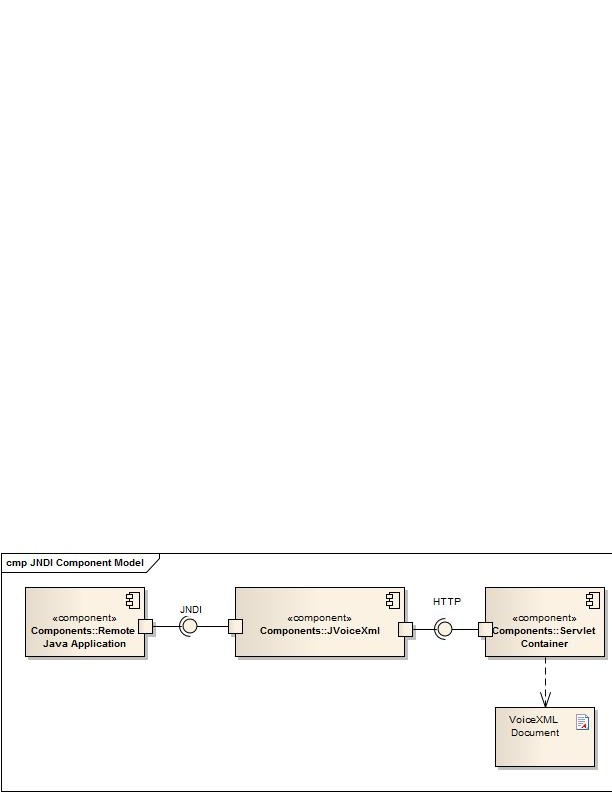
\includegraphics[width=\linewidth]{client-architecture.jpg}
\caption{Basic architecture of JVoiceXML}
\label{fig:architecture}
\end{figure}

Usually, the VoiceXML documents are stored in a web server or a servlet
container and are accessed, e.g., via the HTTP protocol. JVoiceXML also
supports other protocols, e.g. file. In principle all resources can be supported
that can be addressed by a URI scheme, but this will require additional
programming effort. JVoiceXML runs as a
standalone server and retrieves the documents from the servlet container or
other document repository. Some more information can be found in
chapter~\ref{cha:document-server}. 

There are mainly two ways, how clients can interact with JVoiceXML
\begin{inparaenum}[(i)]
\item using JNDI or
\item using the \lstinline{CallMananger.}
\end{inparaenum}

Most of the demo clients use the Java Naming and Directory Interface
(JNDI)~\cite{sun:jndi} to access JVoiceXML. They can also initiate calls for an application using this 
technology. Currently there is only basic telephony support, but users can call 
applications from their own Java programs. This is also the reason, why some
programming effort is needed to start with your first programs. The way this is
done is described in chapter~\ref{cha:programmatic-approach}.

Conceptually JNDI allows to connect to a centralized running JVoiceXML 
server.

JVoiceXML also allows to have all that at the server side with the help of a
\lstinline{CallManager}.
This typical architecture for a voice browser is shown in
figure~\ref{fig:server-architecture}. Here JVoiceXML waits for incoming
calls and once the \lstinline{CallManager} detects an call, it calls the
configured application. This architecture aims at settings where JVoiceXML
is accessed using e.g. SIP or via MMI messages. 
The current demo implementations mainly support JNDI, since the speaker and the
microphone of the JVoiceXML server are used for speech output and input.
Redirection of the audi streams is still in its infancy and may need
custom build implementation platforms.
\begin{figure}
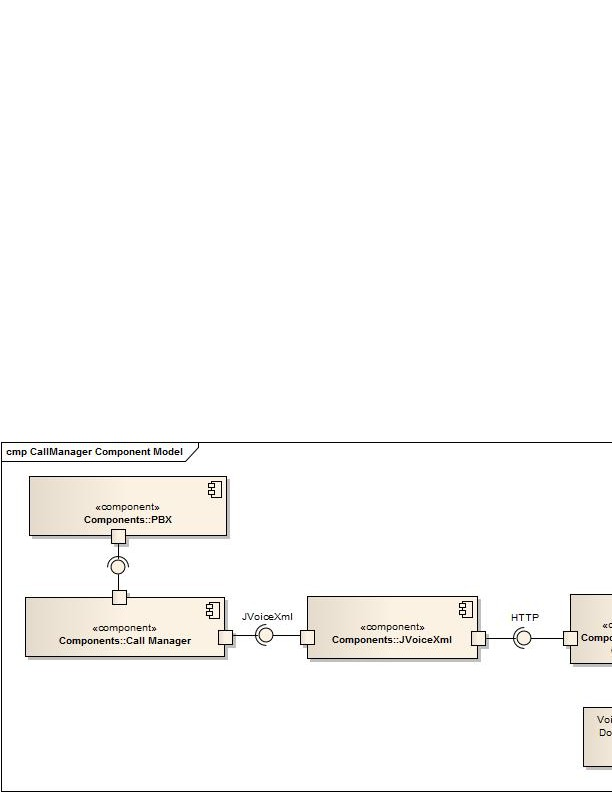
\includegraphics[width=\linewidth]{server-architecture.jpg}
\caption{Architecture of JVoiceXML using a CallManager}
\label{fig:server-architecture}
\end{figure}
This approch is described in more detail in section~\ref{cha:callmanager}.

\section{Required Software}
\label{sec:required-software}

JVoiceXML is written in JAVA and you will at least need a JAVA compiler, an 
editor or preferably a JAVA IDE, see section~\ref{sec:ide}, and ANT, see 
section~\ref{sec:ant}, to build and run the binaries for the 
clients. Tomcat~\cite{apache:tomcat} from the Apache Software Foundation can be
used as a servlet container.

\subsection{IDE}
\label{sec:ide}

You can use the IDE of your choice to edit the sources and compile the 
demos. You can even use a simple text editor to perform this job.
Nevertheless there are some restriction that you cannot work around.

Your IDE must support at least J2SE 1.7. The demos use ANT 1.7 for compilation. 
ANT is not required but used as a means of IDE independent project setup.

\subsection{JAVA}
\label{sec:java}

Parts of the code of JVoiceXML are using features from the JAVA 7 API, so that
you will need at least J2SE 7 to compile the code. You can download it
for free from \url{http://java.sun.com}.

For now, you will need to do some programming to call your applications, but
this is subject of change in later revisions.

\subsection{ANT}
\label{sec:ant}

The demos are being built by an ANT build file to keep it IDE independent. It is
recommended that you use at least ANT 1.7.0. 
If you don't have ANT installed, you can download the current release
from \url{http://ant.apache.org}.

Nearly all IDEs feature an ANT integration. This allows to use the scripts with
your favorite IDE.

The demos of this user guide do not rely on ANT, so you do not need to install
ANT if you play with the examples of this user guide.

\subsection{Tomcat}
\label{sec:tomcat}

VoiceXML is designed to access documents via the HTTP protocol among others. This
guide uses Tomcat 6~\cite{apache:tomcat} for this purpose.
Tomcat can be obtained
from \url{http://tomcat.apache.org}. You can also use the servlet container of
your choice.

It is also possible to store the VoiceXML files in the file system and let
them be processed by JVoiceXML. In that case, you do not need a servlet
container.

\subsection{Implementation Platform Dependent Software}

JVoiceXML is shipped with several implementation platforms. Some may require
additional software as it is described in the following section.

\section{Installation}
\label{sec:installation}

You can download the compiled voice browser as \texttt{jvxml-VERSION.zip} from 
\url{http://jvoicexml.sourceforge.net/downloads.htm}.
\texttt{VERSION} has to be replaced by the used version number, e.g. 0.7.0.GA.
Unpack the zipped distribution file and open a command prompt in that
directory. Call the installer 

\begin{lstlisting}
java -jar jvxml-install-VERSION.jar
\end{lstlisting}

For windows double-clicking the jar should do the trick. 

This will install the browser into a directory of your choice. In the rest of 
this document this directory will be referred as \lstinline{JVOICEXML_HOME}.

JVoiceXML is shipped with different implementation platforms. Install only
those platforms that you intend to use. The configuration issues of each
platform is described in the following sections.

For this user guide, it is recommended to use the text implementation platform
and the JSAPI 2.0 implementation platform with either the SAPI or the
Sphinx/FreeTTS part. It is also possible to install everything and drop those
configuration files from the \lstinline{$JVOICEXML_HOME/config} folder that you do not need. You
can simply create a subfolder \lstinline{unused} in that directory and move the
unused configuration files to this folder. The configuration files follow the
naming convention \lstinline{<platform>-implementation.xml}. The following
section gives a first insight into the available platforms.

\subsection{JSAPI 1.0 implementation platform}

The JSAPI 1.0 implementation platform targets JSAPI 1.0 compliant speech
recognizers and synthesizers. JVoiceXML offers two speech engines for this
platform:
\begin{enumerate}
  \item Talking Java
\end{enumerate}

You will need to install at least one of these engines in order to use this
platform. Note that all options may be displayed, depending on you operating
system.

Thanks to Jontahan Kinnersley, JVoiceXML ships with the Talking Java hook from
from \url{http://www.cloudgarden.com}. This copy is free for
private use. You should buy a license if you use it in a commercial setting.

Talking Java requires an installation of the Microsoft Speech API, which is
already part of Windows Vista and Windows 7. In order to run it on Windows XP
you need to install the speech SDK 5.1 for Windows in advance. It can be
downloaded for free from
\url{http://www.microsoft.com/downloads/en/details.aspx?FamilyID=5e86ec97-40a7-453f-b0ee-6583171b450}.

Note that Talking Java is not compatible with any other JSAPI platform. This
means, that you will have to disable other platforms that are built on top of
JSAPI 1 or 2. Otherwise, the JVM will crash.

\subsection{JSAPI 2.0 implementation platform}

The JSAPI 2.0 implementation platform targets JSAPI 2.0 compliant speech
recognizers and synthesizers. As a first start JVoiceXML is shipped with a
first approach to use Sphinx 4 and FreeTTS with this new API. Additionally,
we added support for the Microsoft Speech API and TTS for Mac OS X.
Note, that this requires Windows 7. Windows Vista or Windows XP are not
supported. 

This is an implementation of a draft specification of JSR 113 developed under
the Java Community Process (JCP) and is made available for testing and evaluation
purposes only. The code is not compatible with any specification of the JCP.

\subsection{JTAPI implementation platform}

The JTAPI implementation platform can be used in addition to any other
implementation platform to enable telephony support. Currently there are some
basic tests in conjunction with the JSAPI 2.0 implementation platform, but this
needs some more furhter programming before it actually can be used.

\subsection{Mary implementation platform}

This implementation platform offers support for the OpenMary speech synthesizer. 
It requires that you have an installed mary on your computer. OpenMary can be
downloaded for free from \url{http://mary.dfki.de}.

This platform can be used in addition to other platforms, e.g. JSAPI 2.0 to
substitute the JSAPI speech synthesizer. Note that you will need to install an
implementation platform featuring a speech recognizer to start JVoiceXML.


\subsection{Marc implementation platform}

This implementation platform offers support for MARC, a talking
head developed by LIMSI. MARC can be downloaded from 
\url{http://marc.limsi.fr}. MARC requires that you have an installed mary on
your computer. OpenMary can be downloaded for free from \url{http://mary.dfki.de}.

This platform can be used in addition to other platforms, e.g. JSAPI 2.0 to
substitute the JSAPI speech synthesizer. Note that you will need to install an
implementation platform featuring a speech recognizer to start JVoiceXML.

\subsection{MRCPv2 implementation platform}

The MRCPv2 implementation platform targets MRCPv2 compliant speech recognizers
and synthesizers. This platform is useful, if you are interested in an easy
integration with commercial server based speech engines.

An open source MRCPv2 implementation is available via the Cairo project. You can
download Cairo from \url{http://cairo.sourceforge.net}. Cairo makes use of JMF
2.1.1e to stream the audio. JMF is available from Oracle at
\url{http://www.oracle.com/technetwork/java/javase/download-142937.html}. Note
that JMF is outdated and does not work with 64bit Java under Windows.
Follow the instructions to install Cairo and JMF. Then, start Cairo. The
connection will not work, if cairo is not present when JVoiceXML starts. 

Before starting JVoiceXML, you need to adapt the settings in
\lstinline{mrcpv2-callmanager.xml}. Adapt the SIP settings and the address of
the Cairo Server. If you did not change anything and if you are running cairo
on the same machine, you can use the following values:
\begin{description}
\item[cairoSipAddress] sip:cairo@speechforge.org
\item[cairoSipHostName] IP address of the cairo server
\item[cairoSipPort] usually 5050
\end{description}

The value for \texttt{mySipAddress} must be set to \texttt{sip:<your IP
address>:4242} with \texttt{<your IP address>} replaced by your real IP address. 
Do not use \texttt{localhost} or 
\texttt{127.0.0.1} but replace it with the real IP address of your machine.

The entry for the \lstinline{applications} of the \lstinline{callmanager}
specify which SIP extension number is associated with which URL to your
VoiceXML application.
An example is shown here:
\begin{lstlisting}[language=XML]
<beans:property name="applications">
  <beans:map>
    <beans:entry key="1000"
      value="http://127.0.0.1:8080/helloworldservletdemo/HelloWorld" />
    <beans:entry key="2000"
      value="http://127.0.0.1:8080/AnotherApp.vxml" />
  </beans:map>
</beans:property>
\end{lstlisting}
In this case, you can call JVoiceXML at 1000 and 2000. If you dial 1000,
JVoiceXML will start to process the \emph{hello world servlet demo}. 
The value can be any URL, e.g. file based URLs.

Note that it may also be necessary to change the RMI port if you are running
Cairo on the same machine as described in section~\ref{sec:jndi-port}.

After the start of JVoiceXML, prepare your softphone to call JVoiceXML.
For our
tests we use x-lite (\url{http://www.counterpath.com/x-lite.html}).
Create a new account and make
sure that the settings are as shown in figure~\ref{fig:sip-properties}.
\begin{figure}
\begin{center}
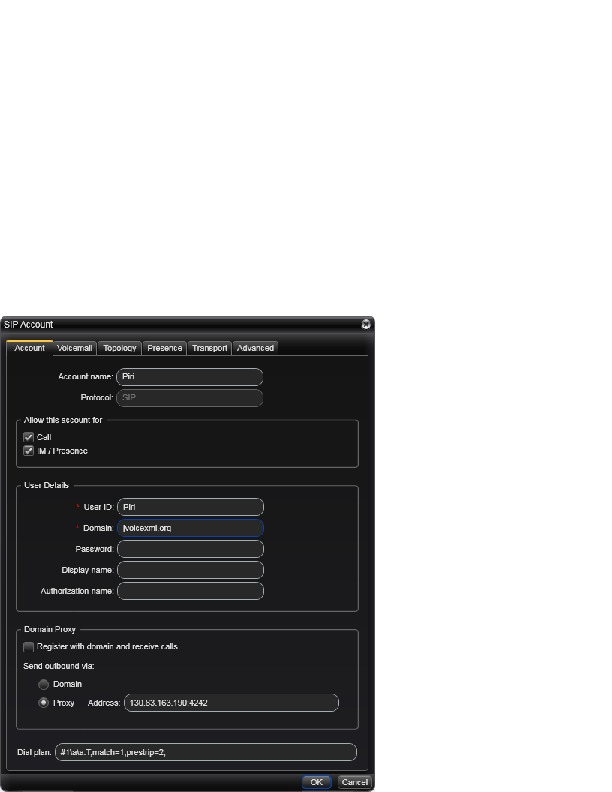
\includegraphics[width=.5\linewidth]{SIPProperties.jpg}
\end{center}
\caption{X-Lite Properties}
\label{fig:sip-properties}
\end{figure}
Make sure, that the Proxy point to the URL of your computer running JVoiceXML
and the port that you configured in the file \texttt{mrcpv2-callmanager.xml}. 
Unselect \emph{Register with domain and receive calls}.

Afterwards you should be able to call JVoiceXML with the number that you
specified in the application configuration.

\subsection{Text implementation platform}

The text implementation platform can be used to have a string based access to
the voice browser. In this case speech recognition and text-to-speech is
replaced by text input and output.

\subsection{MMI CallManager}

JVoiceXML can be used as a modality component in the MMI architectural pattern
which is described at~\cite{w3c:mmi}.

Note that this component only serves as a hook to the MMI system and that you
will need a speech recognizer and a speech synthesizer in addition.

Before starting the MMI call manager you will need to configure the used
implementation platforms in the configuration file \texttt{mmi-callmanager.xml}.
The current demo implementation uses sockets to communicate with JVoiceXML.
However, the used protocol is configurable and may be replaced by own
implementations.

\section{Preparing the first start}
\label{sec:impl-platform-config}

It may be necessary, to install and copy additional software depending on the
implementation platform that you installed. The previous section provided some
hints about it.

All platform configuration files are located in the \lstinline{config} folder.
JVoiceXML scans this folder for configuration files at startup and loads all found
implementation platforms. A full list of the configuration files is
given in section~\ref{sec:configuration-files}. When it starts, JVoiceXML
reports all available platforms in the console window. A possible output is the
following:

\begin{lstlisting}
2467 [JVoiceXmlMain] INFO  ...  available synthesizers:
2467 [JVoiceXmlMain] INFO  ...  - 1 instance(s) of type 'jsapi20'
2467 [JVoiceXmlMain] INFO  ...  - 1 instance(s) of type 'text'
2467 [JVoiceXmlMain] INFO  ...  - 1 instance(s) of type 'mary'
2467 [JVoiceXmlMain] INFO  ...  available recognizers:
2467 [JVoiceXmlMain] INFO  ...  - 1 instance(s) of type 'jsapi20'
2468 [JVoiceXmlMain] INFO  ...  - 1 instance(s) of type 'text'
2468 [JVoiceXmlMain] INFO  ...  available telephones:
2468 [JVoiceXmlMain] INFO  ...  - 1 instance(s) of type 'text'
2468 [JVoiceXmlMain] INFO  ...  - 1 instance(s) of type 'dummy'
\end{lstlisting}

JVoiceXML features a flexible and modular configuration concept. Each
implementation platform can add custom libraries without the need to adapt the
startup script. The following code snippet shows the configuration of the text
based implementation platform as an example.

\begin{lstlisting}[language=XML]
<?xml version="1.0" encoding="UTF-8"?>
<implementation
  xmlns:beans="http://www.springframework.org/schema/beans"
  xmlns:xsi="http://www.w3.org/2001/XMLSchema-instance"
  xsi:noNamespaceSchemaLocation=
    "jvxml-implementation-0-7.xsd">
  <classpath>lib/jvxml-text.jar</classpath>
  <classpath>lib/jvxml-client-text.jar</classpath>
  <beans:bean class=
    "org.jvoicexml.implementation.text.TextPlatformFactory">
    <beans:property name="instances" value="1" />
  </beans:bean>
</implementation>
\end{lstlisting}

This configuration file as well as all the configuration files from the
active implementation platforms can be found in the \lstinline{config} folder.
This configuration introduces two new Java archives to the class loader:
\lstinline{ib/jvxml-text.jar} and \lstinline{ib/jvxml-client-text.jar}.

These jars are added to the CLASSPATH when the platform is loaded.

In addition it is possible to configure certain settings of the platform. In
this case the number of instances is limited to 1. This means that there will be
only one instance of this platform.

A closer look at certain configuration issues is given in
section~\ref{sec:configuration}. 

For the specification of objects JVoiceXML utilizes the spring framework as an
IoC. Please refer to the spring documentation at
\url{http://static.springsource.org/spring/docs/3.1.x/spring-framework-reference/html/}
for more details.

\section{Starting the Voice Browser}

After the installation and possible installation of additional software, the
browser is ready to use. The \texttt{bin} folder contains the files to start
the browser. The relevant files depend on your operating system and are
described in the following sections.

Make sure that you have your configuration right as described in
section~\ref{sec:impl-platform-config}.

JVoiceXML features two modes
\begin{enumerate}
  \item as a server using so called \lstinline{CallManager}s and
  \item controlled by a client program.
\end{enumerate}

The first mode is pretty much what is known from other voice browsers. Here,
you usually initiate a call and JVoiceXML maps the incoming call to a VoiceXML
document. This is explained in more detail in chapter~\ref{cha:callmanager}.

The second mode provides some more control over the execution of a session with
the voice browser. Here, you remotely create a session and specify the VoiceXML
document to process. For now, this is the most advanced and preferred way.
This is explained in more detail in chapter~\ref{cha:programmatic-approach}.

Having started the voice browser it is waiting for incoming requests in either
case. Later on in this guide you will learn how to start sessions
programmatically.

Note, that there is no graphical user interface right now. 

\subsection{Linux}

The shell script \texttt{startup.sh} located in the \texttt{bin} folder
of your JVoiceXML installation can be used to start the browser.

It is written to work independent to the current folder. Simply call

\begin{lstlisting}
sh JVOICEXML_HOME/bin/startup.sh
\end{lstlisting}

On recent Ubuntu and Ubuntu-derived setups, start JVoiceXML using this command:
\begin{lstlisting}
padsp ./startup.sh
\end{lstlisting}

On these systems, pulse is the default audio manager. Using the previously
mentioned way you'll most likely get no
sound, since Java doesn't work properly with alsa (breaks up quickly, calls
the alsa API in stupid ways, so that sound cannot be used by multiple apps
concurrently, locks itself out from using sound etc.), whereas padsp simulates
oss, with which Java works right.


After the start lots of debug information will be displayed.
It may take a while until the TTS engine and the recognizer are launched.
The voice browser can be used, if you see the message

\begin{lstlisting}
VoiceXML interpreter <version> (Revision <number>) started.
\end{lstlisting}

\subsection{Windows}

The windows executable \texttt{JVoiceXML.exe} located in the \texttt{bin}
folder of your JVoiceXML installation can be used to start the browser.
However, the preferred way is to use the batch or shell scripts.
The executable is simply a wrapped Java call and should also work with a
double-click in the windows explorer.

From The command line prompt, call

\begin{lstlisting}
JVOICEXML_HOME\bin\JVoiceXML.exe
\end{lstlisting}

If you start the browser from the windows explorer, a command prompt will open.
After the start lots of debug information will be displayed.
It may take a while until the TTS engine and the recognizer are launched.
The voice browser can be used, if you see the message

\begin{lstlisting}
VoiceXML interpreter <version> (Revision <number>) started.
\end{lstlisting}

\subsection{Troubleshooting}

JVoiceXML should run out of the box. However, it may happen that you discover
problems at startup or while you work with the voice browser. Here the logging
information is a good source to examine the causes. You will realize that there
is a lot of debug information output at the console. Additional output can be
found in the logging folder.

If the level of provided output is not sufficient, you may also lower the level.
Therefore open the file \lstinline{config/log4j.xml} in your favorite editor
and change the line

\begin{lstlisting}[language=XML]
<logger name="org.jvoicexml">
    <level value="info"/>
</logger>
\end{lstlisting}

to

\begin{lstlisting}[language=XML]
<logger name="org.jvoicexml">
    <level value="debug"/>
</logger>
\end{lstlisting}

If this still does not help, do not hesitate to contact the author of this
document. I am always interested in improving the voice browser. This is
easier if I know the problems with it. The preferred way is over the mailing
lists.

If you want to discuss the coding, make suggestions for improvement or if
you have trouble building the binaries, use the
\url{http://lists.sourceforge.net/lists/listinfo/jvoicexml-developer}
developer list.

If you want to get help on our API for your current project, use the
\url{http://lists.sourceforge.net/lists/listinfo/jvoicexml-user} user list.

\section{Shutdown of the Voice Browser}

The \texttt{bin} folder also contains the files to stop the browser. The
relevant files depend on your operating system and are described in the following
sections.

Please avoid to stop the browser using \lstinline{CTRL-C} or by closing the
window. If you have JNDI configured JVoiceXML starts the \lstinline{rmiregistry}.
The registry may not shutdown properly if you closed the voice browser this way
and may keep the configured port active. This will result in some error messages
if you restart JVoiceXML.


\subsection{Linux}

The shell script \texttt{stutdown.sh} located in the \texttt{bin} folder
of your JVoiceXML installation can be used to stop the browser.

It is written to work independent to the current folder. Simply call

\begin{lstlisting}
sh JVOICEXML_HOME/bin/shutdown.sh
\end{lstlisting}

This will make an RMI call to the voice browser and asks it to shutdown.

\subsection{Windows}

The windows executable \texttt{Shutdown.exe} located in the \texttt{bin}
folder of your JVoiceXML installation can be used to stop the browser.

The executable is simply a wrapped Java call and should also work with a
double-click in the windows explorer.

From The command line prompt, call

\begin{lstlisting}
JVOICEXML_HOME\bin\Shutdown.exe
\end{lstlisting}

This will make an RMI call to the voice browser and asks it to shutdown.

\section{Running the Demos}

The browser comes with some demo programs. You'll find them in the
directory \texttt{JVOICEXML\_HOME/demo}. Use the IDE of your choice
and explore there contents. Some features of the browser can 
become more clear with them.

The demos are designed to work with the JSAPI 2.0 implementation platform. Make
sure that you have this configuration enabled before running the demos.

The demo programs feature an ANT script which can be used for starting.
There may be some properties that need to be overwritten in the installed
version. For this purpose there is a template \lstinline{ant.properties} of
relevant properties in the folder \lstinline{JVOICEXML_HOME/demo/config-props}.
To override these properties copy the file \texttt{ant.properties} to the
folder \lstinline{JVOICEXML_HOME/demo/personal-props}. This way you are able
to keep the original settings but also override custom values.

In most cases it should be sufficient to change to each demo directory
and call

\begin{lstlisting}
ant run
\end{lstlisting}

The procedure described above will not work for the
\emph{HelloWorldServletDemo}. In this case you have to add the location of
\texttt{servlet-api.jar} to the \texttt{jvoicexml.properties} by adjusting the
property \texttt{servlet.lib.dir}.

Before you can run this demo, call

\begin{lstlisting}
ant war
\end{lstlisting}

to create a war archive that must be deployed to you servlet container
before running the demo.

The demos are also suitable to get you started with your own first tests.
Currently, the use requires some programming and you could have an easier
start if you reuse the demo code and simply exchange the VoiceXML files.

The following sections will help you to get a better understanding of the
code that is used in the demos.

\chapter{The Document Server}
\label{cha:document-server}

This first example shows how VoiceXML documents are accessed from a
servlet container or a web server and how clients can start the application.

It is also possible to have the VoiceXML files in the file system. In this case
you have to use a URL using the \lstinline{file} scheme, e.g.
\lstinline{file:///home/user/text.vxml}. For this guide we follow the W3C
specification to retrieve the VoiceXML documents via the \lstinline{HTTP}
protocol.

\section{Creating and storing a VoiceXML file}
\label{sec:hello-vxml}

This first example is very simple. It just echos a 'hello world'.
Create a file \texttt{hello.vxml} with the following content:

\begin{lstlisting}[language=XML]
<?xml version="1.0" encoding="UTF-8"?> 
<vxml xmlns="http://www.w3.org/2001/vxml" version="2.1">
  <form>
    <block>Hello World!</block>
  </form>
</vxml>
\end{lstlisting}

Copy this file to a directory of your web server that can be accessed
by a browser. For Tomcat create a directory \texttt{demo1} in
the \texttt{\$CATALINA\_HOME/webapps} directory and copy the VoiceXML
file to this directory. In order to make this
an accessible web application, create the empty sub-folder \texttt{WEB-INF}
in \texttt{demo1}.

Now, try to access the file in your browser. For Tomcat this is
\url{http://localhost:8080/demo1/hello.vxml}. If all went well the
contents of this file is displayed in the browser. In some cases the file
might be offered for download. This is the default behaviour of your browser if
it can not determine the type of the file. Download the file and open it in your
favorite editor to verify that this is your VoiceXML code.


\chapter{JVoiceXML as a Server}
\label{cha:callmanager}

The ususal way to interact with a voice browser would be to run JVoiceXML as a
server and interact with it by issuing calls with a phone. However, the history
of JVoiceXML is not like this so there is still something to do to make this
happen. The most advanced setting here is to have JVoiceXML as a modality
component in an MMI setting~\cite{w3c:mmi}.

Typically this solution needs other implementation platforms in addition. This
may be e.g. JSAPI 2.0. Refer to section~\ref{sec:installation} for a complete
list of available implementation platforms.

Have a closer look at the \lstinline{org.jvoicexml.demo.mmi.simpledemo} for a
start.

\chapter{JVoiceXML Clients}
\label{cha:programmatic-approach}

\section{A first TTS example}
\label{sec:first-tts-example}

This example uses the VoiceXML file that has been coded in
section~\ref{sec:hello-vxml} and shows how it can be synthesized by writing an
own client. 

\subsection{Writing the Client}

A client is a program that remotely calls JVoiceXML and initiates calls.
Typically, this ought to be done by a PBX like Asterisk or FreeSwitch. In
absence of these telephony environments, it might be useful to run
VoiceXML documents on a regular desktop PC. This enables you to play around with
VoiceXML without the need to setup a PBX. The multitude of available
implementation platforms makes it hard to come up with a simple solution that
you can use to simply execute a VoiceXML file. In this section you will learn
how to program your own \emph{generic} test environment. Therefore, create a
Java file \texttt{Demo1.java} with the following content:

\begin{lstlisting}[language=Java]
public class Demo1 {
    public static void main(String[] args) {
    }
}
\end{lstlisting}

First, we need to connect to the JVoiceXML voice browser. JVoiceXML
uses JNDI over RMI~\cite{sun:rmi,sun:rmi_jndi} for this purpose. 
The following code snippet
shows how to obtain a remote reference to the main entry for
all client applications \lstinline[language=Java]{org.jvoicexml.JVoiceXml}:

\begin{lstlisting}[language=Java]
import javax.naming.Context;
import javax.naming.InitialContext;

import org.jvoicexml.JVoiceXml;
...
    public static void main(String[] args) {
        Context context = null;
        try {
            context = new InitialContext();
        } catch (javax.naming.NamingException ne) {
            ne.printStackTrace();
            System.exit(-1);
        }

        JVoiceXml jvxml = null;
        try {
            jvxml = (JVoiceXml) context.lookup("JVoiceXml");
        } catch (javax.naming.NamingException ne) {
            ne.printStackTrace();
            System.exit(-1);
        }
...
\end{lstlisting}

\subsubsection{JNDI Settings}

In line 9, a \lstinline[language=Java]{Context} is created to access JNDI resources.
The settings how to do this are obtained from a file named
\texttt{jndi.properties} which must be in the \texttt{CLASSPATH}.
\texttt{jndi.properties} has the following contents:

\begin{lstlisting}
java.naming.factory.initial=\
    com.sun.jndi.rmi.registry.RegistryContextFactory
java.naming.provider.url=rmi://localhost:1099
java.naming.rmi.security.manager=true
\end{lstlisting}

The location of JVoiceXML is stored in the property 
\texttt{java.naming.pro\-vider.url}. If you want to access JVoiceXML on a 
different computer you have to replace \texttt{localhost} with the IP address 
or name of that computer.

\subsubsection{Required Client Libraries}

The classes  that are required to access JVoiceXML, like
\lstinline[language=Java]{org.jvoicexml.JVoiceXml}, are part of the \texttt{jvxml-client.jar} and
\texttt{org.jvoicexml.xml.jar}, which can be found in the \texttt{lib} folder of
your JVoiceXML installation. This jar contains all classes, that you need to write
client applications. If you are using a different implementation platform, you
may need to add other more specific client jars in addition to these libraries.

Next, we call the browser to process the application. This is done
by creating a \lstinline[language=Java]{org.jvoicexml.Session} object.

\begin{lstlisting}[language=Java]
...
import org.jvoicexml.Session;
...

    public static void main(String[] args) {
        ...
        JVoiceXml jvxml = null;
        try {
            jvxml = (JVoiceXml) context.lookup("JVoiceXml");
        } catch (javax.naming.NamingException ne) {
            ne.printStackTrace();
            System.exit(-1);
        }

        final ConnectionInformation info =
            new BasicConnectionInformation(
                "dummy", "jsapi20", "jsapi20");
        final Session session = 
            jvxml.createSession(info);

        final URI uri;
        try {
            uri = 
          new URI("http://localhost:8080/demo1/hello.vxml");
        } catch (URISyntaxException e) {
            e.printStackTrace();
            System.exit(-1);
        }

        try {
            session.call(uri);

            session.waitSessionEnd();

            session.hangup();
        } catch (org.jvoicexml.event.JVoiceXMLEvent e) {
            e.printStackTrace();
            System.exit(-1);
        }
    }
...
\end{lstlisting}

The argument on the \lstinline[language=Java]{createSession}() is a
\lstinline[language=Java]{ConnectionInformation} object. This object is
responsible for the selection of the implementation platform we are going to
use. An implementation platform features three types of resources:
\begin{itemize}
  \item telephony,
  \item system output and
  \item user input.
\end{itemize}
The resources are identified by strings. In this case, we use a dummy telephony
implementation and system output and user input from the JSAPI 1.0
implementation platform. This combination uses the microphony and speaker of
your PC. Telephony is not needed, so we use the dummy resource. With the call to
\lstinline[language=Java]{jvxml.createSession(info)}, we create a session that
is bound to the given resource types.

The argument for \lstinline[language=Java]{session.call(URI)} must point to to URI of the
root document of your application.

A simplification of the above is available by the
\lstinline{org.jvoicexml.GenericClient}. Here, the code can be reduced to

\begin{lstlisting}[language=Java]
...
import org.jvoicexml.Session;
...
    public static void main(String[] args) {
        ...
        try {
            final URI uri = 
                new URI("http://localhost:8080/demo1/hello.vxml");
            final GenericClient client = new GenericClient();
            final Session session =
                client.call(uri,  "dummy", "jsapi20", "jsapi20");

            session.waitSessionEnd();

            session.hangup();
        } catch (org.jvoicexml.event.JVoiceXMLEvent e) {
            e.printStackTrace();
            System.exit(-1);
        } catch (URISyntaxException e) {
            e.printStackTrace();
            System.exit(-1);
        }
    }
...
\end{lstlisting}

\subsection{Special issues for the text client}

If you are not using the text platform, you can simply skip this section and
continue to start the client as it is described in
section~\ref{sec:starting-the-client}.

The text platform sends the user output to the client and receives user input as
pure text strings. Therefore, we need to sligtly modify our class
\lstinline[language=Java]{Demo1} to implement
\lstinline[language=Java]{org.jvoicexml.client.text.TextListener} from
the Java archive \lstinline{org.jvoicexml.client.text}. 

\begin{lstlisting}[language=Java]
...
import org.jvoicexml.client.text.TextListener;
import org.jvoicexml.xml.ssml.SsmlDocument;
...
public class Demo1 implements TextListener
    public static void main(String[] args) {
        ...
    }

    public void started() {
    }

    public void connected(final InetSocketAddress remote) {
        ...
    }

    public void outputSsml(final SsmlDocument document) {
        ...
    }

    public void disconnected() {
        ...
    }
...
\end{lstlisting}

You will receive the system output in the method
\lstinline[language=Java]{outputSsml(SsmlDocument}. Note, that you will also
need to include the xml library \texttt{org.jvoicexml.xml.jar}. This is, where
the \lstinline[language=Java]{SsmlDocument} is defined.

The communication between JVoiceXML and your client is based on sockets. The
utility class \lstinline[language=Java]{TextServer} helps you to create this
socket, register your \lstinline[language=Java]{TextListener} and create the
required \lstinline[language=Java]{ConnectionInformation}. Therefore, replace
the creation of the \lstinline[language=Java]{ConnectionInformation} by

\begin{lstlisting}[language=Java]
...
    private Object lock = new Object();

    public static void main(String[] args) {
        ...
        JVoiceXml jvxml = null;
        try {
            jvxml = (JVoiceXml) context.lookup("JVoiceXml");
        } catch (javax.naming.NamingException ne) {
            ne.printStackTrace();
            System.exit(-1);
        }

        final TextServer server = new TextServer(4242);
        final Demo1 demo = new Demo1();
        server.addTextListener(demo);
        server.start();
        synchronized (lock) {
            lock.wait();
        }
        final ConnectionInformation info =
            server.getConnectionInformation();
        final Session session = 
            jvxml.createSession(info);

        final URI uri;
        try {
            uri = 
          new URI("http://localhost:8080/demo1/hello.vxml");
        } catch (URISyntaxException e) {
            e.printStackTrace();
            System.exit(-1);
        }
        ...
    }

    public void started() {
        synchronized (lock) {
            lock.notifyAll();
        }
    }
...
\end{lstlisting}

The object \lstinline[language=Java]{lock} is used as a semaphore to delay until
the server started. You will need a similar mechanism to delay after you
initiated a call before you can use the \lstinline{TextServer} to send messages
to your VoiceXML application. Once the \lstinline{connected(...)} of your
\lstinline{TextListener} gets called, it is safe to use.

Again, the code can be simplified through the \lstinline{GenericClient}.
The created \lstinline{ConnectionInformation} can also be used to initiate
calls.
 \begin{lstlisting}[language=Java]
 ...
        final ConnectionInformation info =
            server.getConnectionInformation();
        final Session session = 
            jvxml.createSession(info);
        final URI uri = ...
        ...
        final GenericClient client = new GenericClient();
        final Session session = client.call(uri,  info);
...
\end{lstlisting}

Note, that you will also need to modify the jndi configuration file
\texttt{\${JVOICE-} \texttt{XML\_HOME}/config/jvxml-jndi.xml} to use the text
libraries:

\begin{lstlisting}[language=XML]
<?xml version="1.0" encoding="UTF-8"?>
<jndi xmlns:beans="http://www.springframework.org/schema/beans"
  xmlns:xsi="http://www.w3.org/2001/XMLSchema-instance"
  xsi:noNamespaceSchemaLocation="jvxml-jndi-0-7.xsd">
  <repository>text</repository>
  ...
</jndi>
\end{lstlisting}

Note that a single instance of a \lstinline{TextServer} is only able to handle
a single session. For multiple parallel sessions you will need to use multiple 
\lstinline{TextServer} instances.

\subsection{Starting the Client}
\label{sec:starting-client}

The JNDI implementation of JVoiceXML is based on RMI, and
the implementation for the used interfaces are obtained by
RMI dynamic code download. This means that you have to provide
the location of the library with the implementation of the
interfaces and a security policy file.

For the start this security policy file \texttt{jvoicexml.policy}
allows everything to the remote user:

\begin{lstlisting}
grant {
    permission java.security.AllPermission;
};
\end{lstlisting}

A more restrictive policy can be

\begin{lstlisting}
grant {
  permission java.util.PropertyPermission
      "jvoicexml.vxml.version", "read";
  permission java.util.PropertyPermission
      "jvoicexml.xml.encoding", "read";
  permission java.net.SocketPermission
      "127.0.0.1:1024-", "connect,resolve";
  permission java.io.FilePermission
      "${JVOICEXML_HOME}/lib/-", "read";
};
\end{lstlisting}

The location of the policy is provided by the following environment property

\begin{lstlisting}
-Djava.security.policy=jvoicexml.policy
\end{lstlisting}

Once you start Demo1 it connects to JVoiceXML and starts processing
the application. If you are successful you should hear a synthesized voice
speaking \emph{Hello World}. The application terminates when the processing
finishes.

Depending on your configuration, it may occur that you encounter some weird
\lstinline{ClassCastException}. In this case make sure that you are using the
same classloader repositories for your implementation platform and the
JNDI configuration. See section \ref{sec:classloader-repositories} for
details.

\section{Creating VoiceXML using the Tag Library}

JVoiceXML features a strong tag library to author VoiceXML documents. In
this section we will write a small servlet returning the VoiceXML document that
was used in section~\ref{sec:first-tts-example} using this library.

\subsection{Creating the Servlet}

Our basic seleton for a servlet looks as follows:

\begin{lstlisting}[language=Java]
import java.io.IOException;
import javax.servlet.ServletException;
import javax.servlet.http.HttpServlet;
import javax.servlet.http.HttpServletRequest;
import javax.servlet.http.HttpServletResponse;

public class HelloServlet extends HttpServlet {
    public void doGet(HttpServletRequest request,
        HttpServletResponse response)
        throws ServletException, IOException {
    }
}
\end{lstlisting}

Our code goes into the \lstinline[language=Java]{doGet()} method of the servlet. The tag library
is located in the package \lstinline[language=Java]{org.jvoicexml.xml}. Hence you have to add
\texttt{org.jvoicexml.xml.jar} to the CLASSPATH.

Before using the classes you have to import the required classes by adding
\begin{lstlisting}[language=Java]
import org.jvoicexml.xml.*;
\end{lstlisting}

Then, the VoiceXML document can be created and returned by adding
\begin{lstlisting}[language=Java]
    public void doGet(HttpServletRequest request,
        HttpServletResponse response)
        throws ServletException, IOException {
        Vxml vxml = document.getVxml();
        Form form = vxml.appendChild(Form.class);

        Block block = form.appendChild(Block.class);
        block.addText("Hello World!");

        response.setContentType("text/xml");
        final String xml = document.toXml();
        final PrintWriter out = response.getWriter();
        out.println(xml);
    }
\end{lstlisting}

Each tag has a corresponding class in the tag library and has also convenient
methods to set and get the allowed attributes.

A child tag can be added using the scheme
\begin{lstlisting}[language=Java]
ChildTag child = parentTag.appendChild(ChildTag.class);
\end{lstlisting}

ParentTag and ChildTag have to be replaced by the concrete class. If a child
tag is not allowed for a parent tag, a \lstinline[language=Java]{IllegalArgumentException} is
thrown.

Next we are going to send the created document to the servlet response stream.
This is done by adding the following code right after the document code:

\begin{lstlisting}[language=Java]
response.setContentType("text/xml");
final String xml = document.toString();
final PrintWriter out = response.getWriter();
out.println(xml);
\end{lstlisting}

A string representation of the created document can be obtained via the
\lstinline[language=Java]{toString()} method. JVoiceXML uses the Java API for
XML streaming for this purpose which is part of Java 6.

\subsection{Creating the WAR Archive}

Servlets are distributed as a war archive. The description for the servlet
container, e.g. Tomcat, is located in the \texttt{web.xml} file.
This file has the following content for our example:

\begin{lstlisting}[language=XML]
<?xml version="1.0" encoding="UTF-8"?>

<!DOCTYPE web-app
    PUBLIC
    "-//Sun Microsystems, Inc.//DTD Web Application 2.3//EN"
    "http://java.sun.com/dtd/web-app_2_3.dtd">

<web-app>
    <display-name>JVoiceXML HelloWorld Demo</display-name>
    <description>
        Demo for servlet based VoiceXML creation.
    </description>

    <servlet>
        <servlet-name>JVoiceXMLHelloWorldDemo</servlet-name>
        <servlet-class>
            HelloServlet
        </servlet-class>
    </servlet>

    <servlet-mapping>
        <servlet-name>JVoiceXMLHelloWorldDemo</servlet-name>
        <url-pattern>/helloworld</url-pattern>
    </servlet-mapping>
</web-app>
\end{lstlisting}

The file is stored in the WAR archive \texttt{hello.war}. This archive has the
following structure
\begin{lstlisting}
+- web.xml
+- WEB-IND
   +- classes
      +- HelloServlet.class
   +- lib
      +- org.jvoicexml.xml.jar
\end{lstlisting}

Copy the created war archive to the \texttt{\$CATALINA\_HOME/webapps}
directory and restart Tomcat.

\subsection{Adapting the Code for Demo1}

Demo1 from section~\ref{sec:first-tts-example} has to be adapted to point to
the URL of our servlet. Change the line
\begin{lstlisting}[language=Java]
uri = new URI("http://localhost:8080/demo1/hello.vxml");
\end{lstlisting}
to
\begin{lstlisting}[language=Java]
uri = new URI("http://localhost:8080/hello/helloworld");
\end{lstlisting}

\subsection{Starting the Client}

To start the adapted client follow the steps as they are described in
section~\ref{sec:starting-client}.

\section{Capturing User Input}

This example shows how JVoiceXML can be used to capture user input. 

\subsection{Creating the VoiceXML file}

We use the same environment as introduced in section~\ref{sec:hello-vxml}. Here
we use the source folder \texttt{demo2}.
The demo asks the user a question with the possible answers
\emph{Yes} and \emph{No}.

Our VoiceXML code in the file \texttt{input.vxml} looks like this:

\begin{lstlisting}[language=XML]
<?xml version="1.0" encoding="UTF-8"?> 
<vxml xmlns="http://www.w3.org/2001/vxml" version="2.1"
      xml:base="http://localhost:8080/demo2/">
  <form>
    <field name="answer">
      <grammar src="yesno.srgs" type="application/srgs+xml"/>
      <block>Do you like this example?</block>
      <noinput>
        Please say something.
        <reprompt/>
      </noinput>
      <nomatch>
        Please say yes or no.
        <reprompt/>
      </nomatch>
      <filled>
        <if cond="answer=='yes'">
           You like this example.
        <else/>
           You do not like this example.
        </if>
      </filled>
    </field>
  </form>
</vxml>
\end{lstlisting}

\subsection{Creating the Grammar}
\label{sec:creating-grammar}

The VoiceXML code above relates to the grammar \texttt{yesno.srgs} in 
format~\cite{w3c:srgs}.
It is also possible to have the grammar in SRGS XML format~\cite{w3c:2000:jsgf}.
The grammar format highly depends on the used implementation platform. Some
possible types for the implementation platforms that are shipped with the
browser are shown in Table~\ref{tbl:grammar-types}.

\begin{table}
\begin{center}
\begin{tabular}{|l|l|l|}
\hline
\textbf{Implementation platform} & \textbf{Grammar format} & \textbf{Type} \\
\hline
\hline
JSAPI 1.0 & JSGF & application/x-jsgf \\
\hline
JSAPI 2.0 & SRGS+XML & application/srgs+xml \\
\hline
Text & SRGS+XML & application/srgs+xml \\
\hline
\end{tabular}
\end{center}
\caption{supported grammars per implementation platform}
\label{tbl:grammar-types}
\end{table}


Create a file \texttt{yesno.srgs} with the following content:

\begin{lstlisting}
<?xml version="1.0" encoding="UTF-8"?>
<grammar version="1.0" root="yesno" xml:lang="en"
    xmlns="http://www.w3.org/2001/06/grammar" mode="voice"
    xmlns:xsi="http://www.w3.org/2001/XMLSchema-instance"
    xsi:schemaLocation="http://www.w3.org/2001/06/grammar
        http://www.w3.org/TR/speech-grammar/grammar.xsd"
    tag-format="semantics/1.0">
    <rule id="yesno" scope="public">
        <one-of>
            <item>yes</item>
            <item>no</item>
        </one-of>
    </rule>
</grammar>
\end{lstlisting}

The same grammar in the JSGF format woould look like:

\begin{lstlisting}
#JSGF V1.0;

grammar yesno;
public <yesno> =  yes | no;
\end{lstlisting}

Add the grammar file to you war archive.

\subsection{Writing the Client to Capture Input}

The client for this demo looks pretty much like the client for the \emph{Hello
World!} example.

Copy the file \texttt{Demo1.java} into a file \texttt{Demo2.java} and adapt the
URI to point to the demo2.

\begin{lstlisting}[language=Java]
...
import org.jvoicexml.Session;
...

    public static void main(String[] args) {
        ...
        JVoiceXml jvxml;
        try {
            jvxml = (JVoiceXml) context.lookup("JVoiceXml");
        } catch (javax.naming.NamingException ne) {
	    ne.printStackTrace();
            System.exit(-1);
    }

    final ConnectionInformation info =
        new BasicConnectionInformation(
            "dummy", "jsapi20", "jsapi20");
    final Session session = 
        jvxml.createSession(info);

    final URI uri;
    try {
        uri = 
          new URI("http://localhost:8080/demo2/input.vxml");
    } catch (URISyntaxException e) {
        e.printStackTrace();

        System.exit(-1);
    }

    try {
        session.call(uri);

        session.waitSessionEnd();

        session.hangup();
    } catch (org.jvoicexml.event.JVoiceXMLEvent e) {
        e.printStackTrace();

        System.exit(-1);
    }
...
\end{lstlisting}

\subsection{Special issues for the text client to send input}

For the text client the user input is send to the server as text strings. Again,
the \lstinline[language=Java]{TextServer} utility class helps us with it.
Text input can be delivered by calling:

\begin{lstlisting}[language=Java]
    server.sendInput("yes");
\end{lstlisting}

Take care that the server connected to the client. You will get the
appropriate notifications via the \lstinline[language=java]{TextListener}
methods.

Also note, that you will have to use SRGS+XML formatted grammars.

\subsection{Starting the Client to Capture Input}
\label{sec:starting-the-client}

Start the Demo2 application as you did for Demo1, refer to
section~\ref{sec:starting-client}.

You will be prompted \emph{Do you like this example?}. Now you can answer
either \emph{yes} or \emph{no}. Depending on what you say you will hear the
corresponding statement.

Please use a headset when trying this example. Since the voice browser uses the
speaker and the microphone of your PC it may happen that the output of the
synthesizer is being recognized as your input by mistake.

\section{Builtin Grammars}

In section~\ref{sec:creating-grammar} we manually created the grammar to
define the valid user input. Platforms can support fundamental grammars, the
so-called \emph{built-in} grammars. Currently JVoiceXML provides initial support
for two of them:
\begin{itemize}
  \item boolean
  \item digit
\end{itemize}

The parameters follow the specification of~\cite{w3.org:voicexml} appendix P.
The URL must be of the following form:

\begin{lstlisting}
builtin://<mode>/<type>[?parameters]
\end{lstlisting}

where \emph{mode} is one of \emph{dtmf} or \emph{voice} and \emph{type} denotes
one of the types mentioned above.

An grammar using a boolean type with 7 as the value for \emph{yes} and 9
meaning \emph{no} would look as follows:

\begin{lstlisting}[language=XML]
<grammar src="builtin:dtmf/boolean?y=7;n=9"/>
\end{lstlisting}

Currently, the grammar is generated in SRGS XML format and converted into JSGF
if you are using the JSAPI 1.0 implementation platform. The SRGS grammar
makes use of tags to transform the entered digit into a boolean. This
transformation is current not upported, so JVoiceXML is not able to do the
anlalog transformation for JSGF. As a workaround you will have to check for 7
and 9 in your conditions for this platform. We will have a closer look at the
semantic interpretation in the following section.

This does not apply if you are using the SRGS grammar format.

\section{Semantic Interpretation}
\label{sec:semantic-interpretation}

The previous example used the following comparison to check if the user uttered
\emph{yes}:

\begin{lstlisting}[language=XML]
<if cond="answer=='yes'">
  You like this example.
<else/>
  You do not like this example.
</if>
\end{lstlisting}

This is not very generic, especially, if the user also may want to agree by
saying e.g. \emph{sure}. In order to allow for other options to agree, we need
a mapping mechanism. That is where semantic interpretation comes into play. We
modify the grammar from the previous example to

\begin{lstlisting}
<?xml version="1.0" encoding="UTF-8"?>
<grammar version="1.0" root="yesno" xml:lang="en"
    xmlns="http://www.w3.org/2001/06/grammar" mode="voice"
    xmlns:xsi="http://www.w3.org/2001/XMLSchema-instance"
    xsi:schemaLocation="http://www.w3.org/2001/06/grammar
        http://www.w3.org/TR/speech-grammar/grammar.xsd"
    tag-format="semantics/1.0">
    <rule id="yesno" scope="public">
        <one-of>
            <item>yes<tag>yes</tag></item>
            <item>sure<tag>yes</tag></item>
            <item>no<tag>no</tag></item>
        </one-of>
    </rule>
</grammar>
\end{lstlisting}

Similarly, the JSGF version is

\begin{lstlisting}
#JSGF V1.0;

grammar yesno;
public <yesno> =  yes{true} | yeah{true} | no{false};
\end{lstlisting}

Using this modified grammar, the output of the recognizer will be evaluated
as the boolean values \lstinline{true} and \lstinline{false}. Hence, we are
able to modify the check to

\begin{lstlisting}[language=XML]
<if cond="answer">
  You like this example.
<else/>
  You do not like this example.
</if>
\end{lstlisting}

JSGF has very limited capabilities to enable semantic interpretation.
It allows only the presence of some tag strings. JVoiceXML extends this to
support for boolean values, numbers and strings. Note that you will have to 
enclose the tag into simple quotes \emph{\'} for strings.
The following example will map the utterance to the strings \lstinline{yes}
and \lstinline{no}:
\begin{lstlisting}
#JSGF V1.0;

grammar yesno;
public <yesno> =  yes{'yes'} | yeah{'yes'} | no{'no'};
\end{lstlisting}
which will have be checked as before.

Using SRGS the available options allow for more complex constructs. You can
specify more complex semantic interpretations as explained in the following
section.

\section{Mixed Inititiative Dialogs}

In the previous examples the computer directed the dialog. VoiceXML also allows
to create mixed initiative dialogs, where both, the human and the computer
are able to take control.

A common approach to create a mixed initiative dialog is to use the
\lstinline{<initial>} tag.
This tag is visited when the user is initially being prompted for form-wide
information.
The following example of a simple pizza ordering service may help to understand
how to implement it.

\begin{lstlisting}[language=XML]
<?xml version="1.0" encoding="UTF-8"?>
<vxml version="2.0" xmlns="http://www.w3.org/2001/vxml"
    xmlns:xsi="http://www.w3.org/2001/XMLSchema-instance"
    xsi:schematicLocation=
"http://www.w3.org/2001/vxml http://www.w3.org/TR/voicexml20/vxml.xsd">

    <form id="order">
        <grammar src="pizza.gram"
            type="application/srgs+xml" />

        <block>
            <prompt bargein="false">
                Welcome to the JVoiceXML pizza service!
            </prompt>
        </block>

        <initial name="start">
            <prompt>
                Which pizza do you want?
            </prompt>
            <noinput />
            <nomatch/>
        </initial>
    </form>
</vxml>
\end{lstlisting}

In this example, there is only a single form \lstinline{order} which introduced
a global grammar, makes a short introduction \emph{Welcome to the JVoiceXML
pizza service} before it prompts the user \emph{Which pizza do you want?}.

The grammar may look as follows:
\begin{lstlisting}
<?xml version="1.0" encoding="UTF-8"?>
<grammar version="1.0" root="order" xml:lang="de"
    xmlns="http://www.w3.org/2001/06/grammar" mode="voice"
    xmlns:xsi="http://www.w3.org/2001/XMLSchema-instance"
    xsi:schemaLocation="http://www.w3.org/2001/06/grammar
        http://www.w3.org/TR/speech-grammar/grammar.xsd"
    tag-format="semantics/1.0">
    <rule id="politeness1">
        <item repeat="0-1">
            I want
        </item>
    </rule>

    <rule id="politeness2">
        <item repeat="0-1">
            <item> please </item>
        </item>
    </rule>

    <rule id="size">
        <one-of>
            <item>
                small
                <tag>out = "small";</tag>
            </item>

            <item>
                medium
                <tag>out = "medium";</tag>
            </item>

            <item>
                large
                <tag>out = "big";</tag>
            </item>
        </one-of>
    </rule>

    <rule id="topping">
        <one-of>
            <item>
                salami
                <tag>out = "salami";</tag>
            </item>
            <item>
                ham
                <tag>out = "ham";</tag>
            </item>
            <item>
                mushrooms
                <tag>out = "mushrooms";</tag>
            </item>
        </one-of>
    </rule>

    <rule id="order" scope="public">
        <tag>out = new Object(); out.order = new Object;</tag>
        <ruleref uri="#politeness1" />
        <one-of>
            <item>
                <item repeat="0-1">a</item>
                <ruleref uri="#size" />
                pizza
                <tag>out.order.size = rules.size;</tag>
            </item>
            <item>
                <item repeat="0-1">a</item>
                <item repeat="0-1">pizza with</item>
                <ruleref uri="#topping" />
                <tag>out.order.topping = rules.topping;</tag>
            </item>
            <item>
                <item repeat="0-1">a</item>
                <ruleref uri="#size" />
                <tag>out.order.size = rules.size;</tag>
                pizza with
                <ruleref uri="#topping" />
                <tag>out.order.topping = rules.topping;</tag>
            </item>
        </one-of>
        <ruleref uri="#politeness2" />
    </rule>
</grammar>
\end{lstlisting}

So the user may say something like
\begin{itemize}
  \item \emph{I want a small pizza with salami}
  \item \emph{a large pizza with mushrooms please}
  \item \emph{medium}
  \item \emph{ham}
  \item \ldots
\end{itemize}

The evaluation of the grammar turns this into a compound ECMAScript object like
\begin{lstlisting}
out = {
    "order" : {
        "size" : "medium";
        "topping" : "mushrooms";
    }
}
\end{lstlisting}  

The dialog must be able to store that information into corresponding variables.
Therefore, we extend the VoiceXML code as follows right after the initial tag
was closed:
\begin{lstlisting}[language=XML]
<field name="topping" slot="order.topping">
    <prompt>
        Which topping do you want?
    </prompt>
</field>

<field name="size" slot="order.size">
    <prompt>
        Do you want a small, medium or a large pizza?
    </prompt>
</field>
\end{lstlisting}

Using the \lstinline{slot} attributes of the field, we prepared two slots where
the result of the recognition process should go. The mapping is created from 
the path within the \lstinline{out} object. JVoiceXML will only be able to
map an input to a field if either the field's name matches a property of the
\lstinline{out} object or if the slot matches a possibly nested property. 

Currently, the Sphinx implementation does not support \lstinline{out} objects
per rule but uses a global \lstinline{out} object. The grammar mentioned above
has to be adapted accordingly.

The concept of the tags was extended in JVoiceXML to create a mapping from the
tag strings to the scripting engine. In fact an ECMAScript object
\lstinline{order} is created whose attributes \lstinline{topping} and
\lstinline{size} are assigned the value from the right side of the equation in
the tag. 

If a slot was filled, the corresponding field will be assigned the value. If
only one slot was filled, the second one will remain empty and the interpreter
will continue with that field. Ask for the missing and terminate. 

A dialog may look as follows

\medskip
\speech{System}{Welcome to the JVoiceXML pizza service.}
\speech{System}{Which pizza do you want?}
\speech{User}{Salami}
\speech{System}{Do you want a small, medium or large pizza?}
\speech{User}{Small}
\medskip

If the user enters all data at once, the dialog will be a lot shorter:

\medskip
\speech{System}{Welcome to the JVoiceXML pizza service.}
\speech{System}{Which pizza do you want?}
\speech{User}{I want a small pizza with mushrooms}
\medskip

\section{Calling Java Objects}

The \lstinline[language=XML]{<object>} tag of VoiceXML allows to leave the world
of VoiceXML and get in touch with the environment. JVoiceXML offers support for
this tag and enables you to make calls to your own Java objects.

As an example we use a simple calculator that is able to add two number.
Therefore create a VoiceXML document with the following contents

\begin{lstlisting}[language=XML]
<?xml version="1.0" encoding="UTF-8"?>
<vxml version="2.0" xmlns="http://www.w3.org/2001/vxml"
    xmlns:xsi="http://www.w3.org/2001/XMLSchema-instance"
    xsi:schematicLocation=
"http://www.w3.org/2001/vxml http://www.w3.org/TR/voicexml20/vxml.xsd">

    <form id="add">
        <var name="x" expr="7" />
        <var name="y" expr="5" />

        <object name="calc"
            classid="method://Calculator#add"
            data="http://localhost:8080/objectdemo/">
            <param name="value" expr="x" />
            <param name="value" expr="y" />
        </object>

        <block>
            <prompt>
                <value expr="x"/> + <value expr="y"/>
                = <value expr="calc" />
            </prompt>
        </block>
    </form>
</vxml>
\end{lstlisting}

First two variables $x$ and $y$ are declared and assigned a fixed value. These
numbers are passed as parameters to the object call to the Calculator.

The classid tells us which class should be taken and which method to call. The
signature here is \url{method://<fully qualified class name>#method}.
The location where the class can be found is obtained from the value of the data
attribute. Here, it is obtained from the URL
\url{http://localhost:8080/objectdemo/}. Put an ending / at the end
of the URL.

Next, we code the calculator:
\begin{lstlisting}[language=Java]
public class Calculator {
    public int add(Integer a, Integer b) {
        return a + b;
    }
}
\end{lstlisting}

Note that the class must have a default constructor. Otherwise it will not be
able to be instantiated by JVoiceXML. Currently, arguments have to be passed as
objects. In the example we use the object type \lstinline{Integer} instead of
the primitive type \lstinline{int}.

Create a folder \lstinline{objectdemo} as a subfolder to the \lstinline{webapps}
folder in the Tomcat home directory. Copy the VoiceXML file and the compiled
class into this directory. Again, you will have to create an empty
\lstinline{WEB-INF} folder underneath.

The use of static variables is possible, if you want
to e.g., store some information that has to persist between two calls.

\chapter{Extending JVoiceXML with an own Implementation Platform}

In this section a first cookbook on how to create your own imlementation
platform is presented. Currently there is only some basic content to help you
getting started.


\section{RemoteClient}

A remote client is a data container that holds all the information that is
needed to connect the server side resources. Therefore you have to implement
the \lstinline[language=Java]{org.jvoicexml.RemoteClient} interface. This
container is used to transfer all the information that is needed to connect to
your client application from the JVoiceXML resources to the JVoiceXML server.

The identification of remote clients is based on strings. Choose a unique name
for each of your resource types. It is legal to have the same name for all your
types.

The \lstinline[language=Java]{RemoteClient} object is passed to the external
resources once they are obtained from the pool, see
figure~\ref{fig:get-external-resource-from-pool}. The resources are identified
using the custom string. By calling the
\lstinline[language=Java]{connect(RemoteClient)} method the
\lstinline[language=Java]{RemoteClient} object is delivered to the resource and
can be used to grab the connection information.
\begin{figure}[htp]
\begin{center}
  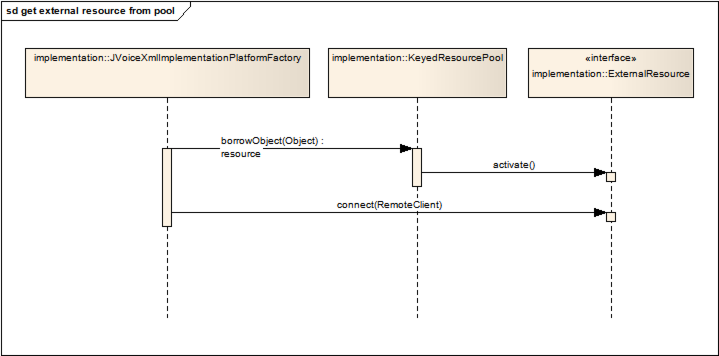
\includegraphics[width=\linewidth]{sd-get-external-resource-from-pool}
  \caption{Get external resource from pool}
  \label{fig:get-external-resource-from-pool}
\end{center}
\end{figure}

Note that \lstinline[language=Java]{RemoteClient} implementations must also
implement \lstinline[language=Java]{java.io.Serializable} to stream the object
from your client to the JVoiceXML voice browser.

\section{Resources}

The first step is to write your own implementations of the resources:
\begin{itemize}
  \item \lstinline[language=Java]{org.jvoicexml.implementation.SpokenInput}
  \item
  \lstinline[language=Java]{org.jvoicexml.implementation.SynthesizedOutput}
  \item \lstinline[language=Java]{org.jvoicexml.implementation.Telephony}
\end{itemize}

Before you start you have to understand the lifecyle of a resource which is
shown in figure~\ref{fig:external-resource-lifecycle}.
\begin{figure}[htp]
\begin{center}
  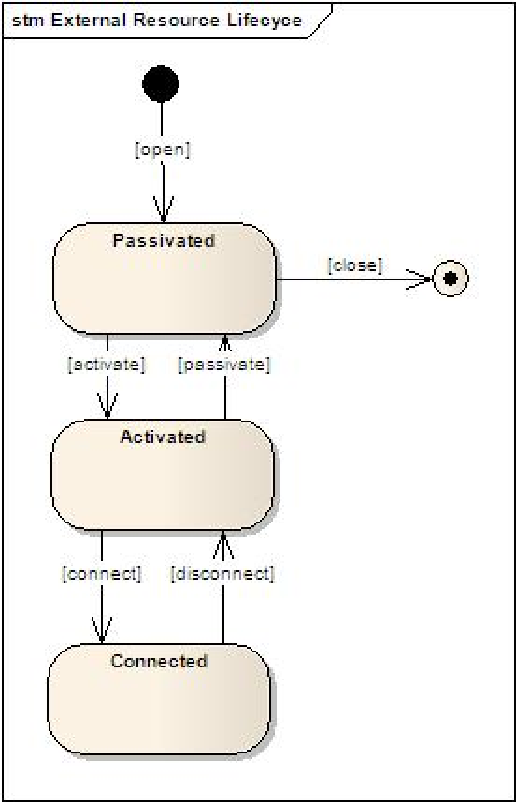
\includegraphics[width=0.4\linewidth]{stm-external-resource-lifecycle}
  \caption{External resource lifecycle}
  \label{fig:external-resource-lifecycle}
\end{center}
\end{figure}
Each transisition is reflected by a corresponding method in the interface
\lstinline[language=Java]{org.jvoicexml.implementation.ExternalResource}
that has to be implemented, see figure~\ref{fig:external-resource}.
\begin{figure}[htp]
\begin{center}
  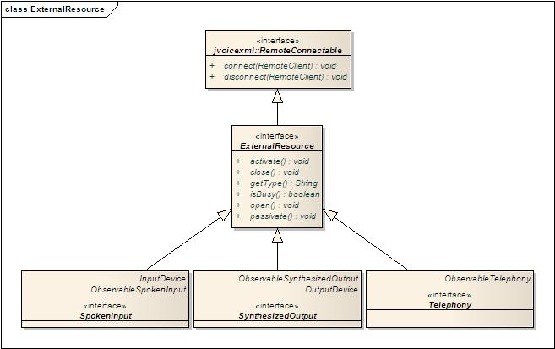
\includegraphics[width=\linewidth]{class-external-resource}
  \caption{External resource inheritance}
  \label{fig:external-resource}
\end{center}
\end{figure}

Your \lstinline[language=Java]{SynthesizedOutput} implementation should maintain
a queue of speakables that should be sent to your client.

Your \lstinline[language=Java]{Telephony} implementation should be able to
conect to your client. It takes the speakables from your Your
\lstinline[language=Java]{SynthesizedOutput} Sending it to your client and also
retrieve inputs from the client. These are forwarded to your 
\lstinline[language=Java]{SpokenInput} implementation. The latter one is
responsible to notify the JVoiceXML voice browser about incoming speech events.

Figure~\ref{fig:play} shows how the voice browser addresses the resources to
queue a \lstinline[language=Java]{Speakable}.
\begin{figure}[htp]
\begin{center}
  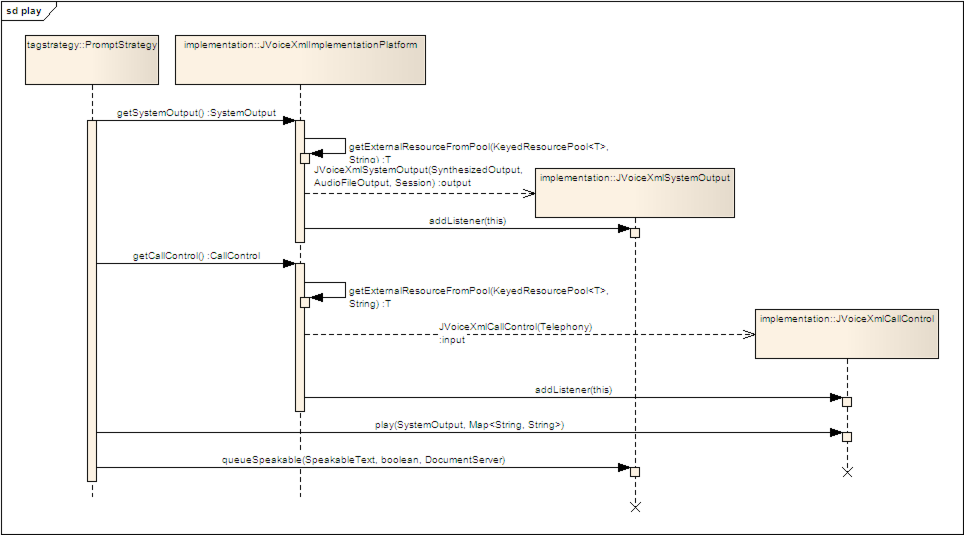
\includegraphics[width=\linewidth]{sd-play}
  \caption{Prompt queuing of the PromptStrategy}
  \label{fig:play}
\end{center}
\end{figure}
JVoiceXML does not make any assumptions how the implementation resources
transfer the \lstinline[language=Java]{Speakable}s from the
\lstinline[language=Java]{SynthesizedOutput} implementation to the
\lstinline[language=Java]{Telephony} implementation. That's why the
\lstinline[language=Java]{SynthesizedOutput} is passed to the
\lstinline[language=Java]{Telephony} implementation as the argument in a
\lstinline[language=Java]{play} call.

The resources communicate with the JVoiceXML voice browser using a
notification mechanism. Hence it is important that the custom resource classes also implement
the corresponding notification interfaces.

\begin{itemize}
  \item the \lstinline[language=Java]{SpokenInput} resource must also implement
  \\
  \lstinline[language=Java]{org.jvoicexml.implementation.ObservableSpokenInput}
  \item the \lstinline[language=Java]{SynthesizedOutput} resource must also
  implement \\
  \lstinline[language=Java]{org.jvoicexml.implementation.ObservableSynthesizedOutput}
  \item the \lstinline[language=Java]{Telephony} resource must also implement \\
  \lstinline[language=Java]{org.jvoicexml.implementation.ObservableTelephony}
\end{itemize}

\subsection{Resource factories}

The implementation platform retrieves the resources via a
\lstinline[language=Java]{org.jvoicexml.implementation.ResourceFactory}.
Implement a factory for each of your resources.

Return the type that you defined in your
\lstinline[language=Java]{RemoteClient} implementation.

\subsection{JVoiceXML configuration}

JVoiceXML retrieves the resource factories via dependency injection from
configuration files that are located in
\lstinline{$JVOICEXML_HOME/config}. Implementation platform configuration files
must use the \lstinline{jvxml-implementation-version.xsd} schema file.
An example is shown below:

\begin{lstlisting}[language=XML]
<?xml version="1.0" encoding="UTF-8"?>
<implementation xmlns:beans=
      "http://www.springframework.org/schema/beans"
  xmlns:xsi="http://www.w3.org/2001/XMLSchema-instance"
  xsi:noNamespaceSchemaLocation=
      "jvxml-implementation-0-7.xsd">
  <repository>text</repository>
  <classpath>dist/jvxml-text.jar</classpath>
  <classpath>dist/jvxml-client-text.jar</classpath>
  <beans:bean class=
    "org.jvoicexml.implementation.text.TextPlatformFactory">
    <beans:property name="instances" value="8" />
  </beans:bean>
</implementation>
\end{lstlisting}

All tags prefixed with \lstinline{beans} are inherited by the SPRING. Custom
tags are \lstinline{classpath} and \lstinline{repository}. The
\lstinline{classpath} tag allows to add your custom jar files and all third
party jar files that are needed by your implementation platform. By default
JVoiceXML uses an own class loader for these jar files. This way it is possible
to have different versions of the same jar in different implementation
platforms at the same time. The \lstinline{repository} tag allows you to
uniquely identify this class loader repository. Sometimes it is necessary to
share the same repository e.g. with a \lstinline[language=Java]{CallManager}.
Note that Java considers two classes loaded from different class loaders as
different classes.

\chapter{Configuration}

\section{Configuration}
\label{sec:configuration}

After the installation, JVoiceXML should run out of the box. However, there may 
be some circumstances, where it is necessary, to adapt the configuration.

\subsection{JNDI Port}
\label{sec:jndi-port}

The remote access for clients is based on RMI, using the default RMI port. This
can conflict with other applications that also use this technology, like JBoss.
You may also want to change the port to run multiple JVoiceXML server instances
on a single machine.

If you want to change the RMI port for JVoiceXML, you have to make changes in 
two configuration files that you can find in the folder 
\texttt{\$JVOICEXML\_HOME/config}.

In the file \texttt{jvxml-jndi.xml} you have to adapt the \texttt{port} 
attribute in following section

\begin{lstlisting}[language=XML]
<?xml version="1.0" encoding="UTF-8"?>
<jndi xmlns:beans="http://www.springframework.org/schema/beans"
  xmlns:xsi="http://www.w3.org/2001/XMLSchema-instance"
  xsi:noNamespaceSchemaLocation="jvxml-jndi-0-7.xsd">
  <repository>text</repository>
  <classpath>lib/org.jvoicexml.jndi.jar</classpath>
  <beans:bean id="org.jvoicexml.JndiSupport"
    class="org.jvoicexml.jndi.JVoiceXmlJndiSupport">
    <beans:property name="registry">
      <beans:bean id="registry"
        class="org.jvoicexml.jndi.JVoiceXmlRegistry">
        <beans:property name="port" value="1099" />
      </beans:bean>
    </beans:property>
  </beans:bean>
</jndi>
\end{lstlisting}

In addition you have to adapt the file \texttt{jndi.properties}.
Change the port to the same value as above.

\begin{lstlisting}
java.naming.provider.url=rmi://localhost:1099
\end{lstlisting}

Do not forget to do the same in the \texttt{jndi.properties} file of your
clients.

\subsection{Classloader Repositories}
\label{sec:classloader-repositories}

In this section, an advanced feature of JVoiceXML's class loader is described.
This may be relevant if you discover problems with the the remote access.

The Java archives that are introduced by the configuration are loaded
in isolated classloader repositories. Java regards two classes to be different if they are
loaded from different classloaders these libraries must share the same
classloader. On the one hand this is an advantage since it offers the opportunity
to have different versions of the same library active in different classloader
repositories, on the other hand this can be a drawback since we want to share the
libraries among different configuration settings, e.g. a callmanager
configuration and an implementation platform configuration. Sharing the same
classloader repository can be achieved by adding the following line to the
configuration file

\begin{lstlisting}[language=XML]
<repository>name</repository>
\end{lstlisting}

\emph{name} should be replaced a proper name for the repository, e.g.
\emph{text} for the text based implementation platform.

Make sure that the loader repository of the JNDI configuration and your
implementation platform use the same repositories. Otherwise, you will get some
strange \lstinline[language=Java]{ClassCastException}s.

\appendix
\chapter{Configuration Files}
\label{sec:configuration-files}

This section includes copies of the configuration files per
implementation platform. Their content can be copied as an XML file
into the config folder. This way, the repsective implementation
platforms can be activated, ,iven that all referenced jars can be found.

\section{JSAPI 1.0 with Talking Java}
\lstinputlisting[language=XML]{../org.jvoicexml.implementation.jsapi10/etc/jsapi10-talking-java-implementation-dist.xml}

\section{JSAPI 2.0 with Sphinx and FreeTTS}
\lstinputlisting[language=XML]{../org.jvoicexml.implementation.jsapi20/etc/jsapi20-implementation-dist.xml}

\section{JSAPI 2.0 with Microsoft SAPI}
\lstinputlisting[language=XML]{../org.jvoicexml.implementation.jsapi20/etc/jsapi20-sapi-implementation-dist.xml}

\section{JTAPI}
\lstinputlisting[language=XML]{../org.jvoicexml.implementation.jtapi/etc/jtapi-implementation-dist.xml}

\section{MARC}
\lstinputlisting[language=XML]{../org.jvoicexml.implementation.marc/etc/marc-implementation-dist.xml}

\section{MARY}
\lstinputlisting[language=XML]{../org.jvoicexml.implementation.mary/etc/mary-implementation-dist.xml}

\section{MMI with HTTP ETL}
\lstinputlisting[language=XML]{../org.jvoicexml.callmanager.mmi.http/etc/mmi-callmanager-http-dist.xml}

\section{MMI with Socket ETL}
\lstinputlisting[language=XML]{../org.jvoicexml.callmanager.mmi.socket/etc/mmi-callmanager-dist.xml}

\section{MMI with umundo ETL}
\lstinputlisting[language=XML]{../org.jvoicexml.callmanager.mmi.umundo/etc/mmi-callmanager-umundo-dist.xml}

\section{MRCPv2}
\lstinputlisting[language=XML]{../org.jvoicexml.implementation.mrcpv2/etc/mrcpv2-callmanager-dist.xml}

\lstinputlisting[language=XML]{../org.jvoicexml.implementation.mrcpv2/etc/mrcpv2-implementation-dist.xml}

\section{Text}
\lstinputlisting[language=XML]{../org.jvoicexml.implementation.text/etc/text-implementation-dist.xml}

\bibliography{userguide}
\bibliographystyle{plain}


\end{document}


% LocalWords:  backgroundcolor lightgray basicstyle numberstyle stepnumber API
% LocalWords:  JVoiceXML VoiceXML APIs JSAPI JTAPI SourceForge JVoice mkdir cd
% LocalWords:  jvxml startup TTS exe Schnelle userguide servlet http JNDI IDE
% LocalWords:  JVoiceXML IDE's vxml xml UTF xmlns webapps args RMI ne lookup
% LocalWords:  InitialContext printStackTrace JVoiceXml jndi CLASSPATH vider IP
% LocalWords:  url localhost ApplicationRegistry uri toURI mue urise jvxmle api
% LocalWords:  createApplication helloworldservlet createSession RMI's
% LocalWords:  jvoicexml HelloWorldServletDemo
